\documentclass[class=report, crop=false, 12pt,a4paper]{standalone}
\usepackage{enumitem}
\usepackage{multicol}
\usepackage{graphicx}
\usepackage{float}
\usepackage{amsmath}
\usepackage{amssymb}
\usepackage{mathtools}
\usepackage{siunitx}
\usepackage{commath}
\usepackage{array}
\usepackage{natbib}
\usepackage[a4paper,width=150mm,top=25mm,bottom=25mm]{geometry}
\setlength{\parindent}{0pt}
\begin{document}
\section{Revision of Fundamental Concepts}
\subsection{Dimensionless Measures}
Reynolds number: 
\begin{gather}
    Re = \frac{Ud}{v}
\end{gather}
Mach number: 
\begin{gather}
    M = \frac{q}{c} = \frac{q}{(\gamma R T)^{\dfrac{1}{2}}}
\end{gather}
Where: 
\begin{itemize}[noitemsep]
    \item $q$ = local flow speed
    \item $U$ = characteristics flow speed
    \item $d$ = characteristic lengthscale
    \item $c$ = either local or characteristic speed of sound
\end{itemize}
The difference between a characteristic and a local measure is important, especially for compressible flows. 
\subsection{Classical Thermodynamics}
First Law of Thermodynamics (change in internal energy, E):
\begin{gather}
    \Delta E = Q - W
\end{gather}
Second Law of Thermodynamics (entropy cannot decrease): 
\begin{gather}
    \dif S = \frac{\dif Q}{T}
\end{gather}
\subsection{Equation of State}
The relationships for a perfect gas are: 
\begin{gather}
    p = \rho R T \\[5pt]
    c_p - c_v = R \\[5pt]
    \dif U = c_p \dif T \\[5pt]
    \dif E = c_v \dif T
\end{gather}
Where E is the internal energy, U is the enthalpy. The isentropic index is: 
\begin{gather}
    \gamma = \frac{c_p}{c_v}
\end{gather}
\begin{figure}[H]
    \centering
    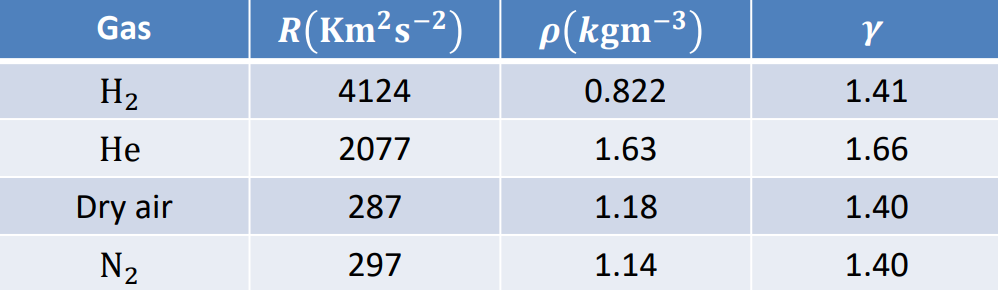
\includegraphics[width = 0.7 \textwidth]{../img/diagram1.PNG} 
    \caption{}
\end{figure}
\subsection{Terminology}
Adiabatic - no heat in / work done (strong changes) \\
Isentropic – no change in entropy (weak changes)
\subsection{Conservation Principles}
There are two frameworks to analyse fluid and solid mechanics.
\begin{figure}[H]
    \centering
    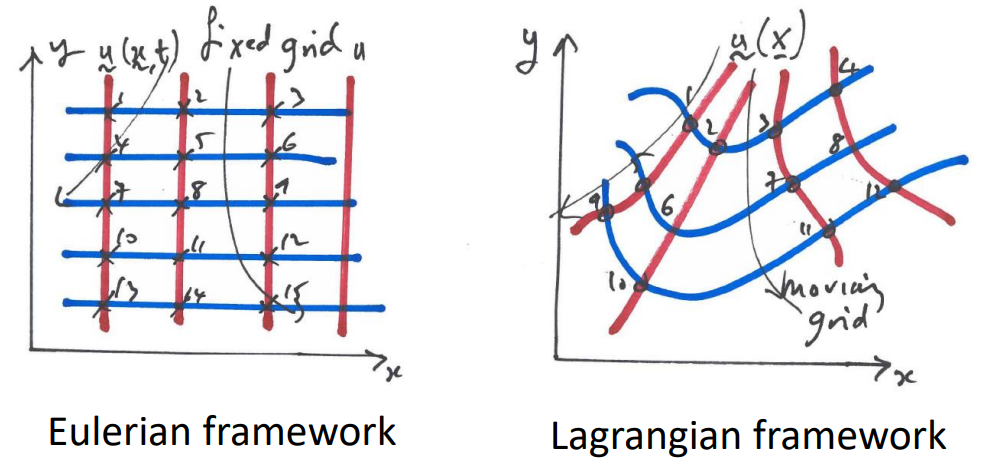
\includegraphics[width = 0.8 \textwidth]{../img/diagram2.PNG} 
    \caption{}
\end{figure}
\begin{itemize}[noitemsep]
    \item Eulerian – information at fixed points
    \item Lagrangian – information at points that move with fluid or solid
    \item They both have advantages and disadvantages.
\end{itemize}
\subsection{Conservation of Mass}Integral form of conservation law for a Lagrangian control volume: 
\begin{gather}
    \frac{\dif}{\dif t}\int_{V_L} \rho \dif V = 0
\end{gather}
Differential form for the conservation of mass: 
\begin{gather}
    \frac{\Dif \rho}{\Dif t} = -\rho(\nabla \cdot u)
\end{gather}
For an incompressible fluid: 
\begin{gather}
    \nabla \cdot u = 0
\end{gather}
\subsection{Conservation of Linear Momentum}
Integral form of the conservation law: 
\begin{gather}
    \frac{\dif}{\dif t} \int_{V_L} \rho u \dif V = \int_{S_L} \sigma \cdot \hat{n} \dif S + \int_{V_L} F \dif V
\end{gather}
Where: 
\begin{itemize}[noitemsep]
    \item $\sigma$ is the stress tensor
    \item $p$ is the pressure 
    \item $\tau$ is the viscous stress tensor
\end{itemize}
\begin{gather}
    \sigma = -pI + \tau
\end{gather}
Differential form of the conservation of momentum: 
\begin{gather}
    \rho \frac{\Dif u}{\Dif t} = \nabla \cdot \sigma + F \\[5pt]
    \rho (x,t) \left( \frac{\partial u}{\partial t} + (u\cdot \nabla)u \right) = -\nabla p
\end{gather}
This is Euler’s equation for an inviscid fluid.
The flow is compressible (explicitly stated). 
\subsection{Conservation of Angular Momentum}
Integral form of the conservation law: 
\begin{gather}
    \frac{\dif}{\dif t}\int_{V_L} \rho x \times u \dif V = \int_{S_L} x \times \sigma \cdot \hat{n} \dif S + \int_{V_L} x \times F \dif V
\end{gather}
The differential form of the conservation law: 
\begin{gather}
    x \times \left( \rho \frac{\Dif u}{\Dif t} - \nabla \cdot \sigma \right) = \epsilon_{ilk}\sigma_{kl}
\end{gather}
Consequence is that the stress tensor is symmetric: 
\begin{gather}
    \sigma_{ij} = \sigma_{ji}
\end{gather}
\subsection{Conservation of Energy}
\begin{gather}
    \frac{\dif}{\dif t} \int_{V_L} \rho \left( E + \frac{1}{2}q^2 \right) \dif V = -\int_{S_L} u \cdot \sigma \cdot \hat{n} \dif S + \int_{S_L} k \nabla T \cdot \hat{n} \dif S + \int_{V_L} u \cdot F \dif V \\[5pt]
    E_T = E + \frac{1}{2}q^2
\end{gather}
Where $q = \abs{u}$ is the fluid speed. The differential form of the energy equation is: 
\begin{gather}
    \rho \frac{\Dif}{\Dif t} \left( E + \frac{1}{2}q^2 \right) = -\nabla \cdot (u \cdot \sigma) + \nabla \cdot (k\nabla T) + u \cdot F
\end{gather}
The continuum form on the conservation of energy says: 
\begin{gather}
    \frac{\Dif E}{\Dif t} = -\frac{p}{\rho}(\nabla\cdot u) + \frac{1}{\rho}(\phi + \nabla \cdot (k\nabla T)) \\[5pt]
    \frac{\Dif E}{\Dif t} = -\dfrac{pD\left(\dfrac{1}{\rho}\right)}{\Dif t} + \frac{\phi + \nabla \cdot (k\nabla T)}{\rho}
\end{gather}
The dissipation is: 
\begin{gather}
    \phi = \nabla \cdot (u\sigma) - u\cdot \nabla \sigma
\end{gather}
Compare to the differential form that you have met before: 
\begin{gather}
    \dif E = -p \dif \left(\frac{1}{\rho}\right) + \dif Q
\end{gather}
For an inviscid fluid (with no viscous dissipation $\sigma = -pI$) and no diffusion of heat: 
\begin{gather}
    \frac{\Dif}{\Dif t} \left( E + \frac{1}{2}q^2 \right) = -\frac{1}{\rho}\nabla \cdot (pu)
\end{gather}
\subsection{Bernoulli’s Equation}
\begin{figure}[H]
    \centering
    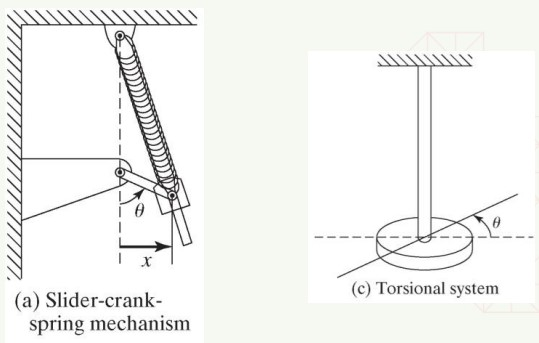
\includegraphics[width = 0.95 \textwidth]{../img/diagram3.PNG} 
    \caption{}
\end{figure}
\subsection{Reference State (Stagnation)}
There are two possible reference states. 
\subsubsection{(a) Stagnation flow condition}
\begin{gather}
    \frac{\gamma}{\gamma - 1} \frac{p}{\rho} + \frac{1}{2}q^2 = const
\end{gather}
The speed of sound is $c$ where: 
\begin{gather}
    c^2 = \left( \frac{\partial p}{\partial \rho} \right)_s = \gamma R T = \frac{\gamma p}{\rho} \\[5pt]
    \frac{p}{\rho} \left( 1 + \frac{1}{2}(\gamma-1)M^2 \right) = const \\[5pt] 
    T \left( 1 + \frac{1}{2}(\gamma - 1)M^2 \right) = const
\end{gather}
We can set the reference constant to be when the flow is a rest or stagnant. For flows where changes are significant, this state cannot be realised without other processes occurring, so that: 
\begin{gather}
    1 + \frac{1}{2}(\gamma - 1)M^2 = \frac{T_0}{T}
\end{gather}
This tells: 
\begin{gather}
    1 + \frac{1}{2}(\gamma - 1)M^2 = \frac{p_0 \rho}{p \rho_0}
\end{gather}
This relationship is not useful, unless combined with the isentropic relationship $\dfrac{p}{\rho^{\gamma}} = const$: 
\begin{gather}
    \frac{p}{p_0} = \left( 1 + \frac{1}{2}(\gamma-1)M^2 \right)^{-\dfrac{\gamma}{\gamma-1}} \\[5pt]
    \frac{\rho}{\rho_0} = \left( 1 + \frac{1}{2}(\gamma-1)M^2 \right)^{-\dfrac{1}{\gamma-1}} 
\end{gather}
\subsubsection{(b) Sonic flow condition} 
\begin{gather}
    \frac{p_{*}}{p_0} = \left( \frac{2}{\gamma+1} \right)^{\dfrac{\gamma}{\gamma-1}} = 0.5283 \\[5pt]
    \frac{\rho_{*}}{\rho_0} = \left( \frac{2}{\gamma+1} \right)^{\dfrac{1}{\gamma-1}} = 0.63 \\[5pt] 
    \frac{T_{*}}{T_0} = \frac{2}{\gamma+1} = 0.8333
\end{gather}
\section{Normal Shocks}
\subsection{Assumptions}
The flow adjusts over a short distance from one region to another and the streamlines are parallel and not deflected.
\\\\
This is called a normal shock. The distance can be very short (comparable with the mean-free path, $10 \mu m$) so that the thickness of the wave may be ignored. Although viscous effects may be important within the wave, an inviscid analysis can be applied to understand these processes. We consider the flow across a shock wave and denote the flow properties with 1 upstream and 2 downstream.
\subsection{Conservation Principles}
Conservation of mass: 
\begin{gather}
    \nabla \cdot (\rho u) = 0
\end{gather}
Conservation of momentum: 
\begin{gather}
    \rho u \cdot \nabla u + \nabla p = 0
\end{gather}
Conservation of energy: 
\begin{gather}
    \rho u \cdot \nabla \left( E + \frac{1}{2}q^2 \right) + \nabla \cdot (pu) = 0
\end{gather}
To apply these relationships we have to integrate them across the shock. Remember, the gradient of these variables is zero on each side because the changes are confined to the thin shock. 
\begin{figure}[H]
    \centering
    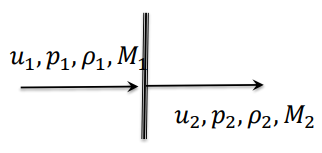
\includegraphics[width = 0.5 \textwidth]{../img/diagram4.PNG} 
    \caption{}
\end{figure}
\begin{gather}
    \rho_2 u_2 = \rho_1 u_1 \\[5pt]
    \rho_2 u_2^2 + p_2 = \rho_1 u_1^2 + p_1 \\[5pt]
    \frac{\gamma}{\gamma - 1} \frac{p_2}{\rho_2} + \frac{1}{2}u_2^2 = \frac{\gamma}{\gamma - 1} \frac{p_1}{\rho_1} + \frac{1}{2}u_1^2 \\[5pt]
    \frac{p_1}{\rho_1 T_1} = \frac{p_2}{\rho_2 T_2}
\end{gather}
Strength of shock is: 
\begin{gather}
    \frac{p_2}{p_1}
\end{gather}
\subsection{Frame of Reference}
\begin{figure}[H]
    \centering
    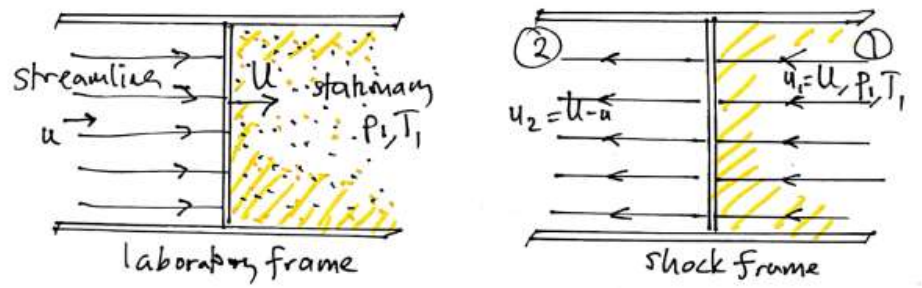
\includegraphics[width = 0.9 \textwidth]{../img/diagram5.PNG} 
    \caption{Diagram showing the frame of reference for an example question}
\end{figure}
When we consider scenarios such as shocks propagating in stationary flows, like a bomb or a pressure pulse is moving into a stationary region, we don't investigate it in this complex form. 
We hop on a frame of reference of the shock so the flow tends to be steady, and then we can conduct an analysis on this framce of reference. 
\subsection{Solution Technique}
Aim of the calculation is to relate the flow upstream of the shock to downstream of the shock. 
There are 4 equations: mass, momentum, energy and state. 
One useful way to solve this is to use 3 of them at a time. 
The systems are solved in pairs: 
\begin{enumerate}[label=(\alph*), noitemsep]
    \item mass, momentum and state (Rayleigh flow) - This occurs in when heat is added to a flow 
    \item mass, energy and state (Fanno flow) - This occurs in when pipe friction is important
\end{enumerate}
\subsection{Algebraic Manipulation}
From the momentum equation: 
\begin{gather}
    p_1 - p_2 = \rho_2 u_2^2 - \rho_1 u_1^2 = \rho_1 u_1 (u_2-u_1)
\end{gather}
Rearranging gives: 
\begin{gather}
    u_2^2 - u_1^2 = \frac{(p_1-p_2)(u_1+u_2)}{\rho_1 u_1} = (p_1-p_2) \left( \frac{1}{\rho_1} + \frac{1}{\rho_2} \right) \\[5pt]
    \frac{2\gamma}{\gamma-1} \left( \frac{p_1}{\rho_1} - \frac{p_2}{\rho_2} \right) = (p_1-p_2) \left( \frac{1}{\rho_1} + \frac{1}{\rho_2} \right)
\end{gather}
Rankine-Hugoniot relation: 
\begin{gather}
    \frac{\rho_2}{\rho_1} = \frac{\left(\dfrac{\gamma+1}{\gamma-1}\right)\dfrac{p_2}{p_1}+1}{\dfrac{p_2}{p_1} + \dfrac{\gamma+1}{\gamma-1}}
\end{gather}
The strength of the shock is: 
\begin{gather}
    \frac{p_2}{p_1} = \frac{\left(\dfrac{\gamma+1}{\gamma-1}\right)\dfrac{\rho_2}{\rho_1}-1}{\dfrac{\gamma+1}{\gamma-1} - \dfrac{\rho_2}{\rho_1}}
\end{gather}
This relationship is valid of shocks and highly non-linear behaviour. 
The first point in the discussion is what happens when the shock is weak. 
\subsection{Weak Shocks}
This can be demonstrated analytically by considering changes of pressure and density across the shock. 
To show this, let $p_2 = p_1 + \Delta p$ and $\rho_2 = \rho_1 + \Delta \rho$, then substituting into the Rankine-Hugoniot gives: 
\begin{gather}
    \frac{\Delta p}{p_1} = \frac{p_2-p_1}{p_1} = \frac{\dfrac{2\gamma(\rho_2-\rho_1)}{(\gamma-1)\rho_1}}{\dfrac{2}{\gamma-1}} = \frac{\gamma\Delta \rho}{\rho_1}
\end{gather}
which is the same as the isentropic approximation obtained by taking the differential of $\frac{p}{\rho^\gamma} = const.$
\\\\
We can write $\rho u^2$ as $\rho c^2 M^2 = \gamma p M^2$. 
Thus the momentum equation may be written as: 
\begin{gather}
    p_1 - p_2 = \gamma p_2 M_2^2 - \gamma p_1 M_1^2
\end{gather} 
or 
\begin{gather}
    \frac{p_2}{p_1} = \frac{1+\gamma M_1^2}{1+\gamma M_2^2}
\end{gather}
The density ratio is: 
\begin{gather}
    \frac{\rho_1}{\rho_2} = \frac{p_2}{p_1} \left( \frac{M_2}{M_1} \right)^2
\end{gather}
This is known as the \textbf{Rayleigh line}. 
\\\\
Since there is no change in stagnation temperature across the shock: 
\begin{gather}
    \frac{T_2}{T_1} = \frac{1+\dfrac{1}{2}(\gamma-1)M_1^2}{1+\dfrac{1}{2}(\gamma-1)M_2^2}
\end{gather}
From the equations of continuity and state: 
\begin{gather}
    \frac{T_2}{T_1} = \frac{p_2 \rho_1}{p_1 \rho_2} = \frac{p_2 u_2}{p_1 u_1} = \frac{p_2 M_2}{p_1 M_1} \left(\frac{T_2}{T_1}\right)^{\frac{1}{2}} \\[5pt]
    \frac{T_2}{T_1} = \left( \frac{p_2}{p_1} \frac{M_2}{M_1} \right)^2
\end{gather}
Substituting into the equation of state gives: 
\begin{gather}
    \frac{p_2}{p_1} = \frac{M_1}{M_2} \left( \frac{1+\dfrac{1}{2}(\gamma-1)M_1^2}{1+\dfrac{1}{2}(\gamma-1)M_2^2} \right)^{\frac{1}{2}}
\end{gather}
This is known as the \textbf{Fanno line}. 
\\\\
Matching the solutions to the Fanno and Rayleigh lines gives the combined solution to the mass, momentum, energy conservation equations and the equation of state: 
\begin{gather}
   \frac{M_1 \left( 1+\dfrac{1}{2}(\gamma-1)M_1^2 \right)^{\frac{1}{2}}}{1+\gamma M_1^2} = \frac{M_2 \left( 1+\dfrac{1}{2}(\gamma-1)M_2^2 \right)^{\frac{1}{2}}}{1+\gamma M_2^2}
\end{gather}
The solutions to this are: 
\begin{gather}
    M_1 = M_2 \\[5pt]
    M_2^2 = \frac{1+\dfrac{1}{2}(\gamma-1)M_1^2}{\gamma M_1^2 - \dfrac{1}{2}(\gamma-1)}
\end{gather}
Note that for $M_1 = M_2 = 1$ there is no shock. For upstream supersonic flows $M_1>1$, the downstream flow is subsonic $M_2<1$. 
\begin{figure}[H]
    \centering
    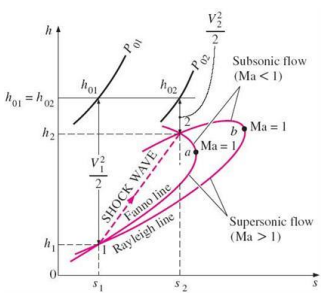
\includegraphics[width = 0.55 \textwidth]{../img/diagram6.PNG} 
    \caption{}
\end{figure}
The pressure and density ratios are important: 
\begin{gather}
    \frac{p_2}{p_1} = \frac{2\gamma M_1^2}{\gamma+1}-\frac{\gamma-1}{\gamma+1} \\[5pt]
    \frac{\rho_2}{\rho_1} = \frac{\dfrac{1}{2}(\gamma+1)M_1^2}{1+\dfrac{1}{2}(\gamma-1)M_1^2}
\end{gather}
Stagnation pressure values can be calculated from: 
\begin{gather}
    \frac{p_{20}}{p_{10}} = \frac{p_{20}}{p_{2}}\frac{p_2}{p_1}\frac{p_1}{p_{10}}
\end{gather}
where the relationship been static and stagnation pressures have been defined. 
\subsection{Entropy Considerations}
From the conservation of energy: 
\begin{gather}
    \dif Q = \dif E + \dif W = c_v\dif T + pd\left(\frac{1}{\rho}\right)
\end{gather}
Since: 
\begin{gather}
    \dif S = \frac{\dif Q}{T}= \frac{c_v \dif T}{T} + \frac{p}{T}d\left(\frac{1}{\rho}\right) = \frac{c_v+R}{T}\dif T - R\frac{\dif p}{p}
\end{gather} 
Integrating gives an entropy change of: 
\begin{gather}
    \Delta s = \int_{1}^{2}\dif s = c_p \log\left(\frac{T_2}{T_1}\right) - R\log\left(\frac{p_2}{p_1}\right) = c_p\log \left( \frac{T_2}{T_1} \left(\frac{p_1}{p_2}\right)^{\dfrac{\gamma-1}{\gamma}} \right)
\end{gather}
Since $c_p = \dfrac{\gamma R}{\gamma-1}$, we can rearrange as: 
\begin{gather}
    \frac{\Delta s}{R} = \frac{\gamma}{\gamma-1} \left( \log\left(\frac{\rho_1}{\rho_2}\right) + \frac{1}{\gamma}\log\left(\frac{p_2}{p_1}\right) \right)
\end{gather}
Specifically for a shock: 
\begin{gather}
    \frac{\Delta s}{R} = \frac{\gamma}{\gamma-1}\log \left( \frac{2}{(\gamma+1)M_1^2} + \frac{\gamma-1}{\gamma+1} \right) + \frac{1}{\gamma-1}\log \left( \frac{2\gamma M_1^2}{\gamma+1} - \frac{\gamma-1}{\gamma+1} \right)
\end{gather}
When $M_1<1$, $M_2>1$ and $\Delta s<0$. This is unphysical and is ignored. But when $M_1>1$, $M_2<1$ and $\Delta s>0$. 
\begin{figure}[H]
    \centering
    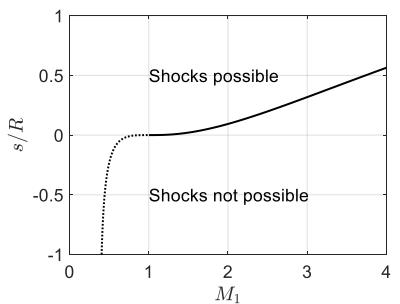
\includegraphics[width = 0.55 \textwidth]{../img/diagram7.PNG} 
    \caption{}
\end{figure}
\subsection{$T-s$ and $p-{1/\rho}$ Diagrams}
We use these types of figures to analyse systems.
\begin{figure}[H]
    \centering
    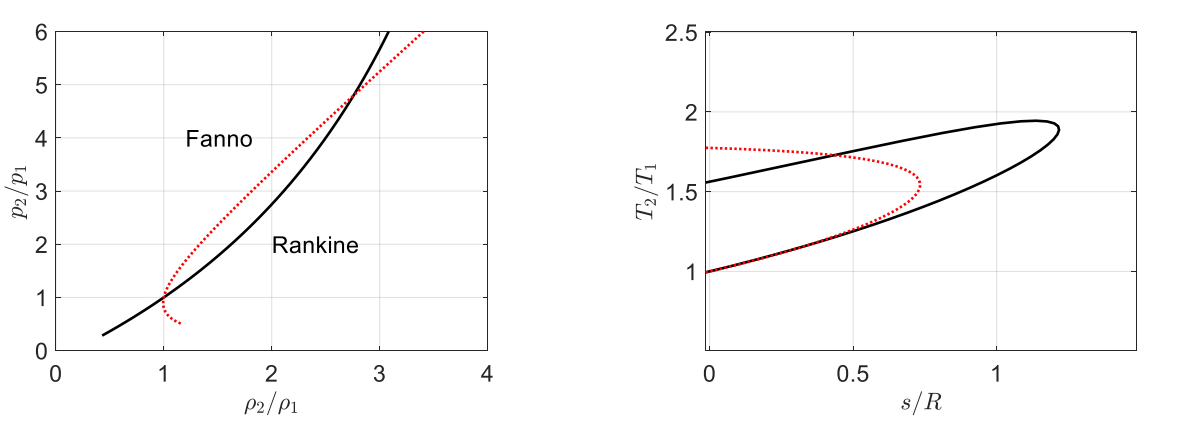
\includegraphics[width = 1 \textwidth]{../img/diagram8.PNG} 
    \caption{}
\end{figure}
\begin{figure}[H]
    \centering
    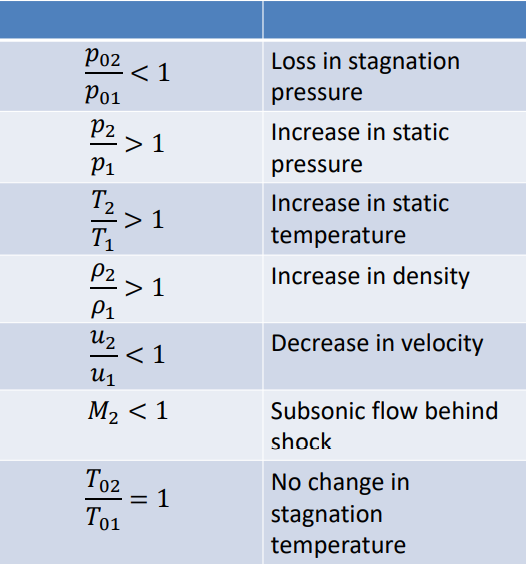
\includegraphics[width = 0.5 \textwidth]{../img/diagram9.PNG} 
    \caption{}
\end{figure}
\end{document}